\section{Introduction}

End user programmers' develop by interleaving opportunistic information foraging with writing code~\cite{brandt_two_2009}~\cite{brandt_example-centric_2010}.
As online coverage of common APIs grows~\cite{parnin_measuring_2011}, programmers increasingly use \emph{crowd documentation} like StackOverflow and blog postings.
Such documentation can be written by coders who lack interest or expertise in writing usable documentation.
Both experienced programmers~\cite{duala-ekoko_asking_2012} and end-user programmers~\cite{dorn_lost_2013}\cite{dorn_learning_2010} struggle to leverage web documentation to solve programming problems.

Decades of research on technical communication provide best practices for writing usable documentation.
In the domain of learning to use software, \emph{minimalist instruction}~\cite{carroll_nurnberg_1990} recommends enabling users to start immediatedly on realistic tasks, reducing the amount of reading and other passive activity, and supporting error recognition and recovery.
Farkas introduces \emph{layered documentation} as an extension to minimalist instruction that enables users from different backgrounds to benefit from the same documents by providing optional \emph{backup information} for tasks like error recognition and correction~\cite{farkas_layering_1998}.

Instructions for web scraping code assumes a reader has some \emph{base literacy} in Python, CSS selectors, and regular expressions.
Given the \emph{diverse backgrounds of both the audience and authors}, it is impractical for the author to introduce all relevant parts of each language in detail.
As a result, today's Q\&A's and blogs lack immediate scaffolding for readers seeking clarification on unfamiliar or complex syntax.

To enable this scaffolded documentation, we propose routines called \emph{\Glspl{name}} that produce on-demand, context-relevant descriptions of specific programming languages, libraries, and commands.
The descriptions are \emph{on-demand} in that they can describe code found anywhere, including the browser or IDE, to provide just-in-time understanding of code.
They are also \emph{context-relevant}, describing only the syntactic elements that are present and important within a snippet.
This distinguishes these explanations from getting-started guides and reference documentation for a language.
Context relevance is defined uniquely for each \gls{name}, as we describe below.

Such explanations can describe languages like CSS selectors and regular expressions.
Each explainer is programmed with several hundred lines of code that \emph{parses} some input code and \emph{generates natural language explanations}.
We show that they be integrated as bookmarklets into a programmer's browser to provide just-in-time explanations of a language, command or API anywhere on the web.
With additional effort, \glspl{name} can generate text descriptions at multiple levels of detail, which we also demonstrate.

Our contributions are as follows.
First, we show a need for micro-explanations by exposing \emph{unexplained languages} in code snippets from popular StackOverflow questions.
Second, we introduce a framework for building a natural language explainer for describing a programming language or command line.
Third, we demonstrate the technical effort required to build \glspl{name} by building them for CSS selectors, command lines, and regular expressions.
Finally, we show through an in-lab study how \gls{name}-generated explanations can help programmers modify existing code containing CSS selectors to perform new tasks when they have no prior knowledge of selectors. \marti{I'm not loving the heavy use of italics in this section.}

\begin{figure}[!t]
\centering{
    \subfigure[Text augmentation explaining a CSS selector]{
        \framebox{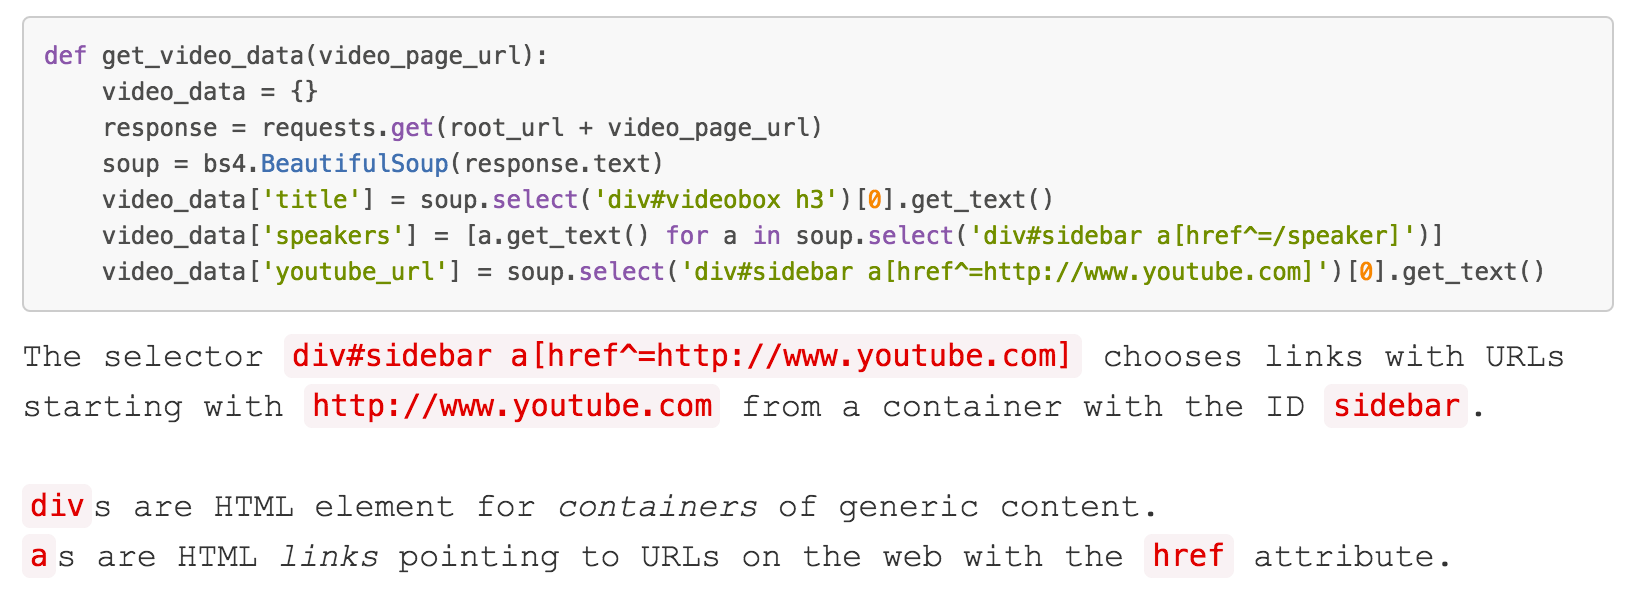
\includegraphics[width=.4\textwidth]{figures/css_explanation}}
        \label{fig:css_explanation}
    }
}
\label{fig:tutorons}
\caption{Automatic, context-relevant textual and visual explanations of code generated by descriptive \glspl{name}.}
\end{figure}
